\chapter{Einleitung}
Die Verwendung von Geräten zum Erfassen von Tastatur-Eingabesequenzen, sogenannten Keyloggern, ist schon seit Mitte der 1970er Jahre publik \cite{engelberg}. Die New York Times berichtete zu dieser Zeit von einer Spionage durch solche Geräte in US-Botschaften und -Konsulaten in Moskau und St. Petersburg, bei welcher IBM Selectric typewriter angegriffen wurden. Es existieren derzeit sowohl Software- als auch Hardware-Keylogger, jedoch lassen sich diese auch noch einmal in verschiedene Unterkategorien unterteilen. So ist z.B. ein Adapter, welcher zwischen Tastatur und PC steckt, wie in Abbildung \ref{keylogger_ps2} \cite{keylogger_ps2} oder \ref{keylogger_usb} \cite{keylogger_usb} dargestellt, eine mögliche Implementierung eines Hardware-Keyloggers. Diese existieren sowohl für PS/2- als auch USB-Tastaturen und sind im Handel frei erhältlich \cite{keelog}.
\begin{figure}
  \centering
  \begin{minipage}{0.45\textwidth}
    \centering
    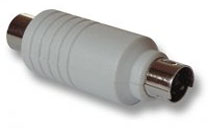
\includegraphics[width=0.6\textwidth]{images/keylogger_ps2.jpg}
    \caption{Keylogger PS/2}
    \label{keylogger_ps2}
  \end{minipage}
  \begin{minipage}{0.45\textwidth}
    \centering
    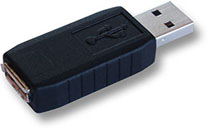
\includegraphics[width=0.6\textwidth]{images/keylogger_usb.jpg}
    \caption{Keylogger USB}
    \label{keylogger_usb}
  \end{minipage}
\end{figure}

Allerdings gelten auch andere Geräte als Hardware-Keylogger, wie z.B. Keypads, welche bei Geldautomaten über das PIN-Feld gelegt werden um den PIN-Code zu erfassen \cite{kirk}. Über Schäden verursacht durch Keylogger existieren allerdings nur wenige Informationen, da Straftaten im Bereich Computerbetrug und Spionage oftmals nicht erkannt oder nicht gemeldet werden \cite{bundeskriminalamt}. So können nur beispielhaft monetäre Erwartungswerte über Schwarzmärkte und spezielle Betrugsdelikte, wie z.B. Kreditkartenbetrug gebildet werden \cite{holz}, oder es werden einzelne Straftaten publik, wie u.a. der versuchte Raub von \$423 Millionen in London \cite{keizer}.

Jedoch ist nicht nur das Mitlesen von Tasteneingaben über die Tastaturschnittstelle möglich, sondern auch die Wiedergabe von Tastatur-Eingabesequenzen, wie u.a. auf der Blackhat Conference demonstriert wurde \cite{chen}. Hierbei wurde die Firmware des Mikrocontrollers derart überschrieben, dass sie nach einer Tasteneingabe und einem zusätzlichen Befehl die Eingabe nochmals in umgekehrter Reihenfolge widergab.

Die vorliegende Bachelorarbeit mit dem Titel ``Aufnahme und Wiedergabe von Tastatur-Eingabesequenzen mittels Arduino Mikrocontroller'' soll jeweils durch eine Implementierung zeigen, dass es einerseits möglich ist Signale einer PS/2-Tastatur mithilfe des Arduino Mikrocontroller \cite{arduino} abfangen und speichern zu können. Andererseits soll gezeigt werden, dass es möglich ist Tastatursignale durch den Mikrocontroller an ein Betriebssystem senden zu können.

Im Folgenden wird sowohl die Idee hinter diesem Thema, als auch mögliche Anwendungen zur Motivation näher beschrieben. Anschließend wird die geplante Herangehensweise für die Bearbeitung dieser Aufgabe geschildert.



\section{Motivation}
Das Aufnehmen und Wiedergeben von Tastatur-Eingabesequenzen bietet viele Möglichkeiten zur Implementierung von nützlichen Funktionalitäten. Im Rahmen dieser Bachelorarbeit dienen drei dieser Funktionalitäten als Motivation und werden dementsprechend mithilfe des Arduino Mikrocontroller \cite{arduino} implementiert:

Die erste Funktionalität ist das einfache Aufzeichnen und Abspeichern der Tastatur-Eingabesequenzen. Dabei sollen die Aufzeichnungen auf einer SD-Karte gespeichert werden, welche beliebig ausgetauscht werden kann.

Als zweite Funktionalität ist das Senden von Tastatursignalen an das Betriebssystem gedacht, welche als Skript auf einer SD-Karte hinterlegt sein können. Nach dem Aufrufen einer Konsole mittels Tastaturkürzeln, die abhängig vom jeweiligen Betriebssystem sind, kann so jeglicher Befehl auf dem System ausgeführt werden. Durch den Einsatz der SD-Karte sind die Skripte austauschbar, sodass verschiedenste Anwendungsmöglichkeiten bestehen.

Die dritte Funktionalität beinhaltet auch das Senden von Tastatursignalen an das Betriebssystem, jedoch werden diese über Ethernet an den Mikrocontroller übertragen. Dies ermöglicht, sofern der Zugriff auf eine Konsole möglich ist, die Steuerung eines Betriebssystems in Echtzeit. Damit gleicht diese Funktionalität einem Remote-Zugriff, jedoch ohne den Einsatz von Software auf dem zu steuernden Betriebssystem.

Da es sich bei den letzten beiden Funktionalitäten um das Senden von Tastatursignalen über das PS/2-Protokoll handelt, besteht weiterhin die Möglichkeit, dass die eingegebenen Befehle ohne eine explizite Prüfung des Betriebssystems oder eines Virenscanners ausgeführt werden können. Dies zu evaluieren ist somit ein weiterer Bestandteil dieser Bachelorarbeit und kann mit Folgen für die IT-Sicherheit verbunden sein.



\section{Aufbau der Arbeit}
Zu Beginn dieser Bachelorarbeit ist im ersten Kapitel die Recherche bezüglich der PS/2-Tastaturschnittstelle und des PS/2-Protokolls für das weitere Vorgehen erforderlich . Zudem werden verwandte Arbeiten aus dem Bereich der Aufnahme und Wiedergabe von Tastatureingabesquenzen beschrieben und die rechtlichen Grundlagen benannt. Im nächsten Kapitel wird die Implementierung der Funktionalitäten dokumentiert. Dies deckt sowohl die notwendigen Softwarekomponenten für den Arduino Mikrocontroller ab, als auch den Aufbau der Elektronik. In dem darauf folgenden Kapitel werden die Ergebnisse der Implementierung evaluiert und bestehende Abwehrmechanismen beschrieben. Abschließend wird in dem letzten Kapitel die Bachelorarbeit zusammengefasst und ein Ausblick für zukünftige Arbeiten gegeben.